%\documentclass[honours,12pt,twoside]{unswthesis}

\usepackage{afterpage}
\usepackage{amsfonts}
\usepackage{amsmath}
\usepackage{amssymb}
\usepackage{amsthm}
\usepackage[english]{babel}
\usepackage{graphicx}
\usepackage{natbib}
\usepackage[utf8]{inputenc}
\usepackage{latexsym}
\usepackage{url}
\usepackage{todonotes}
\usepackage{tikz}
\usepackage{pdfpages}
\usetikzlibrary{arrows}
\usepackage{float}

\usepackage{booktabs}
\renewcommand{\arraystretch}{1.2}


%%%%%%%%%%%%%%%%%%%%%%%%%%%%%%%%%%%%%%%%%%%%%%%%%%%%%%%%%%%%%%%%%
%
%  The following are some simple LaTeX macros to give some
%  commonly used letters in funny fonts. You may need more or less of
%  these
%
\newcommand{\R}{\mathbb{R}}
\newcommand{\Q}{\mathbb{Q}}
\newcommand{\C}{\mathbb{C}}
\newcommand{\N}{\mathbb{N}}
\newcommand{\F}{\mathbb{F}}
\newcommand{\PP}{\mathbb{P}}
\newcommand{\T}{\mathbb{T}}
\newcommand{\Z}{\mathbb{Z}}
\newcommand{\B}{\mathfrak{B}}
\newcommand{\BB}{\mathcal{B}}
\newcommand{\M}{\mathfrak{M}}
\newcommand{\X}{\mathfrak{X}}
\newcommand{\Y}{\mathfrak{Y}}
\newcommand{\CC}{\mathcal{C}}
\newcommand{\E}{\mathbb{E}}
\newcommand{\cP}{\mathcal{P}}
\newcommand{\cS}{\mathcal{S}}
\newcommand{\A}{\mathcal{A}}
\newcommand{\ZZ}{\mathcal{Z}}

%%%%%%%%%%%%%%%%%%%%%%%%%%%%%%%%%%%%%%%%%%%%%%%%%%%%%%%%%%%%%%%%%%%%%
%
% The following are much more esoteric commands that I have left in
% so that this file still processes. Use or delete as you see fit
%
\newcommand{\bv}[1]{\mbox{BV($#1$)}}
\newcommand{\comb}[2]{\left(\!\!\!\begin{array}{c}#1\\#2\end{array}\!\!\!\right)
}
\newcommand{\Lat}{{\rm Lat}}
\newcommand{\var}{\mathop{\rm var}}
\newcommand{\Pt}{{\mathcal P}}
\def\tr(#1){{\rm trace}(#1)}
\def\Exp(#1){{\mathbb E}(#1)}
\def\Exps(#1){{\mathbb E}\sparen(#1)}
\newcommand{\floor}[1]{\left\lfloor #1 \right\rfloor}
\newcommand{\ceil}[1]{\left\lceil #1 \right\rceil}
\newcommand{\hatt}[1]{\widehat #1}
\newcommand{\modeq}[3]{#1 \equiv #2 \,(\text{mod}\, #3)}
\newcommand{\rmod}{\,\mathrm{mod}\,}
\newcommand{\p}{\hphantom{+}}
\newcommand{\vect}[1]{\mbox{\boldmath $ #1 $}}
\newcommand{\reff}[2]{\ref{#1}.\ref{#2}}
\newcommand{\psum}[2]{\sum_{#1}^{#2}\!\!\!'\,\,}
\newcommand{\bin}[2]{\left( \begin{array}{@{}c@{}}
				#1 \\ #2
			\end{array}\right)	}
%
%  Macros - some of these are in plain TeX (gasp!)
%
\newcommand{\be}{($\beta$)}
\newcommand{\eqp}{\mathrel{{=}_p}}
\newcommand{\ltp}{\mathrel{{\prec}_p}}
\newcommand{\lep}{\mathrel{{\preceq}_p}}
\def\brack#1{\left \{ #1 \right \}}
\def\bul{$\bullet$\ }
\def\cl{{\rm cl}}
\let\del=\partial
\def\enditem{\par\smallskip\noindent}
\def\implies{\Rightarrow}
\def\inpr#1,#2{\t \hbox{\langle #1 , #2 \rangle} \t}
\def\ip<#1,#2>{\langle #1,#2 \rangle}
\def\lp{\ell^p}
\def\maxb#1{\max \brack{#1}}
\def\minb#1{\min \brack{#1}}
\def\mod#1{\left \vert #1 \right \vert}
\def\norm#1{\left \Vert #1 \right \Vert}
\def\paren(#1){\left( #1 \right)}
\def\qed{\hfill \hbox{$\Box$} \smallskip}
\def\sbrack#1{\Bigl \{ #1 \Bigr \} }
\def\ssbrack#1{ \{ #1 \} }
\def\smod#1{\Bigl \vert #1 \Bigr \vert}
\def\smmod#1{\bigl \vert #1 \bigr \vert}
\def\ssmod#1{\vert #1 \vert}
\def\sspmod#1{\vert\, #1 \, \vert}
\def\snorm#1{\Bigl \Vert #1 \Bigr \Vert}
\def\ssnorm#1{\Vert #1 \Vert}
\def\sparen(#1){\Bigl ( #1 \Bigr )}

\newcommand\blankpage{%
    \null
    \thispagestyle{empty}%
    \addtocounter{page}{-1}%
    \newpage}
    
%%%%%%%%%%%%%%%%%%%%%%%%%%%%%%%%%%%%%%%%%%%%%%%%%%%%%%%%%%%%%%
%
% These environments allow you to get nice numbered headings
%  for your Theorems, Definitions etc.  
%
%  Environments
%
%%%%%%%%%%%%%%%%%%%%%%%%%%%%%%%

\newtheorem{theorem}{Theorem}[section]
\newtheorem{lemma}[theorem]{Lemma}
\newtheorem{proposition}[theorem]{Proposition}
\newtheorem{corollary}[theorem]{Corollary}
\newtheorem{conjecture}[theorem]{Conjecture}
\newtheorem{definition}[theorem]{Definition}
\newtheorem{example}{Example}
\newtheorem{remark}[theorem]{Remark}
\newtheorem{question}[theorem]{Question}
\newtheorem{notation}[theorem]{Notation}
\numberwithin{equation}{section}

%\begin{document}

\chapter{Convolutional neural networks}\label{convnets}

Convolutional neural networks (\textsc{cnn}s) are of particular interest when working with image problems as the input data is assumed to be two-dimensional. In regular neural networks (see Chapter \ref{neuralNets-intro}), the neurons in each layer are connected to all the neurons of the previous layer. These layers are known as \textit{fully connected layers}. In \textsc{cnn}s, convolutional layers examine only small subimages of the entire image sample. Each pixel of an image forms a neuron, which is connected to nearby pixels and not all pixels of the image. The \textsc{cnn} is trained to identify a set of visual features which can be combined and interpreted for image classification tasks.

% Diagram of typical CNN structure
\begin{figure}[ht]
	\centering
	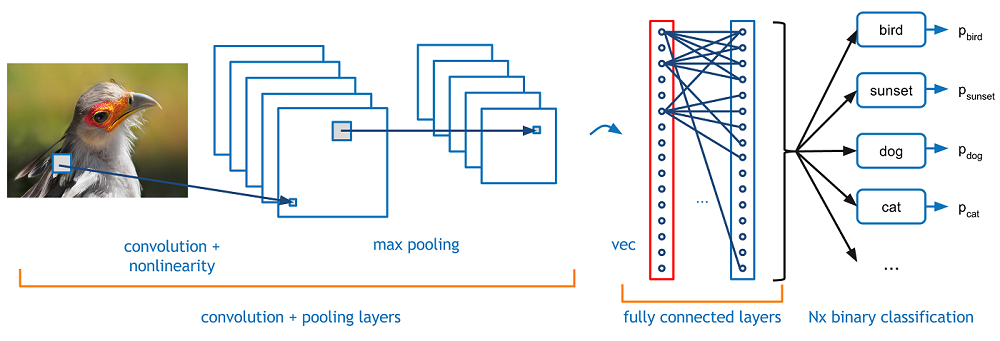
\includegraphics[width=\textwidth]{Images/4_cnn_structure.png}
	\caption{Typical CNN Structure. Convolution layers with ReLU activation (nonlinearity) are followed by pooling layers. The final layers are fully connected, using softmax activation to generate a probability distribution.}
	\small Image taken from \cite{ADeshpande2016}
	\label{convnets-structurefig}
\end{figure}

CNNs typically consist of alternating convolutional layers (see Section \ref{convnets-convlayer}) and max pooling layers (see Section \ref{convnets-pool}), as shown in Figure \ref{convnets-structurefig}. The convolutional layers identify significant visual features, however they introduce a large number of variables into the network. Max pooling layers occur after convolutional layers to reduce network dimensionality. For classification tasks, the last layers of the network are fully connected to restructure the variables as a one-dimensional vector. Softmax activation is used for the final output layer to generate a probability distribution.

\section{Convolutional layers}\label{convnets-convlayer}

The neurons of convolutional layers have a similar overall structure to that of regular neurons (see Section \ref{nnets-structure}). The input variables $X$ are multiplied with weights $W$, summed and added to a bias variable $b$. The resulting linear combination is passed through an activation function $\sigma(\cdot)$ to give the output of the neuron, activation value $a$.

The major difference between convolutional layers and regular neural network layers is the structure of the inputs and weights. Image data is two-dimensional and generally has multiple colour \textit{channels}. For example, a coloured image contains three channels: red, green, and blue. The intensity of each pixel in each channel is represented as a number such that the image forms a three-dimensional array. 

The weights of convolutional layers are formatted as three-dimensional arrays to accommodate for the number of colour channels. These weight arrays are element-wise multiplied with a subset of the whole image. Unlike fully connected layers, convolutional layers do not apply weights to all of the input variables at once. Instead, the weights have an array height and width much smaller than that of the input image, designed to identify particular visual features in smaller subimages. A single matrix of weights that describes a feature is called a \textit{filter}. Each convolutional layer can have multiple filters, analogous to having multiple neurons in a fully connected layer.

The filters are said to \textit{convolve} around the image, multiplying with subimages chosen sequentially, starting from the top-left of the image, and moving towards the bottom-right. Let the $f$-th filter of the convolultional layer be $F^{(f)}$, with dimension $M\times N \times C$. Given an input image matrix $X$, number of channels $C$, and the bias of the $f$-th filter $b^{(f)}$, the value of the convolution at element $X_{j,k}$ is given by
\begin{align}
	a_{jk}^{(f)} = \sigma\left(\sum_{c=1}^C\sum_{m=0}^{M-1}\sum_{n=0}^{N-1}X_{j+m, k+n, c}F_{m,n,c}^{(f)}  + b^{(f)}\right).
\end{align}


\begin{example}
Consider the following simple convolution.
%\begin{figure}[h]
%\centering
%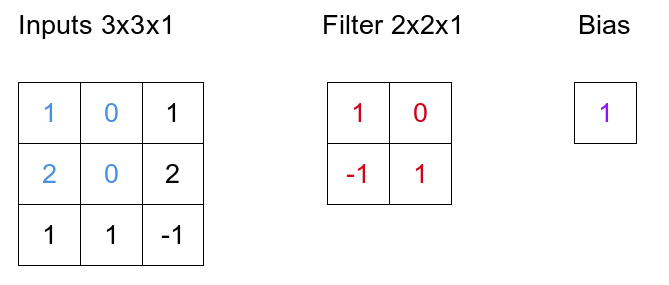
\includegraphics[scale=0.5]{Images/4_conv_eg2.png}
%\label{convnets-conv-eg}
%\end{figure}

\begin{figure}[h]
\centering
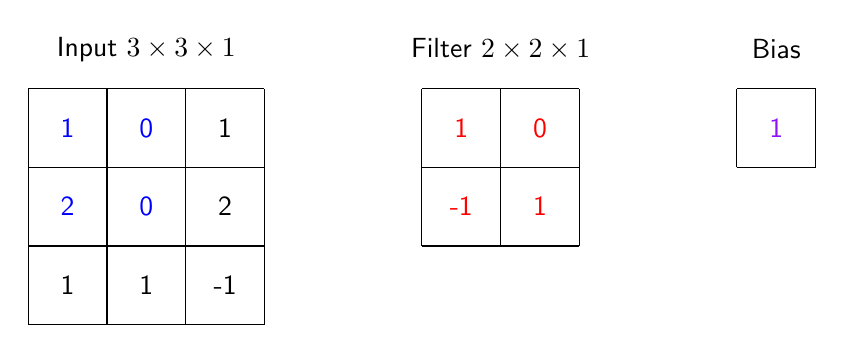
\begin{tikzpicture}[font=\sffamily]
\draw[step=1cm] (0, 0) grid (3, 3);
\draw[step=1cm] (5, 1) grid (7, 3);
\draw[step=1cm] (9, 2) grid (10, 3);

\node at (0.5, 2.5) {\color{blue}1};
\node at (1.5, 2.5) {\color{blue}0};
\node at (2.5, 2.5) {1};
\node at (0.5, 1.5) {\color{blue}2};
\node at (1.5, 1.5) {\color{blue}0};
\node at (2.5, 1.5) {2};
\node at (0.5, 0.5) {1};
\node at (1.5, 0.5) {1};
\node at (2.5, 0.5) {-1};

\node at (5.5, 2.5) {\color{red}1};
\node at (6.5, 2.5) {\color{red}0};
\node at (5.5, 1.5) {\color{red}-1};
\node at (6.5, 1.5) {\color{red}1};

\node at (9.5, 2.5) {\textcolor[rgb]{0.56,0.07,1}{1}};

\node at (1.5, 3.5) {Input $3\times3\times1$};
\node at (6, 3.5) {Filter $2\times2\times1$};
\node at (9.5, 3.5) {Bias};

\end{tikzpicture}
\end{figure}

The filter in red is multiplied element-wise with the inputs given in blue. This gives:
\begin{figure}[h]
\centering
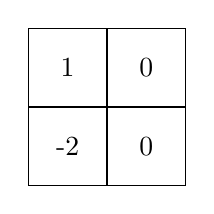
\begin{tikzpicture}
\draw[step=1cm] (0,0) grid (2, 2);
\node at (0.5,1.5) {1};
\node at (1.5,1.5) {0};
\node at (0.5,0.5) {-2};
\node at (1.5,0.5) {0};
\end{tikzpicture}
\end{figure}

Taking the sum of the products and adding the bias in purple gives the activation value $(1 + 0 + -2 + 0) + 1 = 0$. This process is iterated for all $2\times2$ subimages in the original input, giving the following output:

\begin{figure}[h]
\centering
%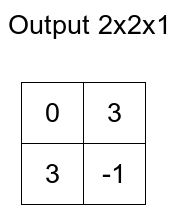
\includegraphics[scale=0.5]{Images/4_conv_eg2_2.png}
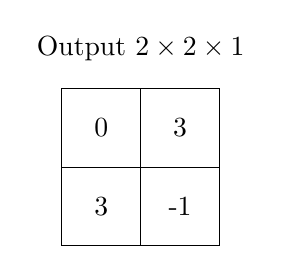
\begin{tikzpicture}

\draw[step=1cm] (0,0) grid (2, 2);
\node at (0.5,1.5) {0};
\node at (1.5,1.5) {3};
\node at (0.5,0.5) {3};
\node at (1.5,0.5) {-1};

\node at (1, 2.5) {Output $2\times2\times1$};

\end{tikzpicture}
\end{figure}

\end{example}

% Diagram of convolution algorithm
%\begin{figure}[ht]
%	\centering
%	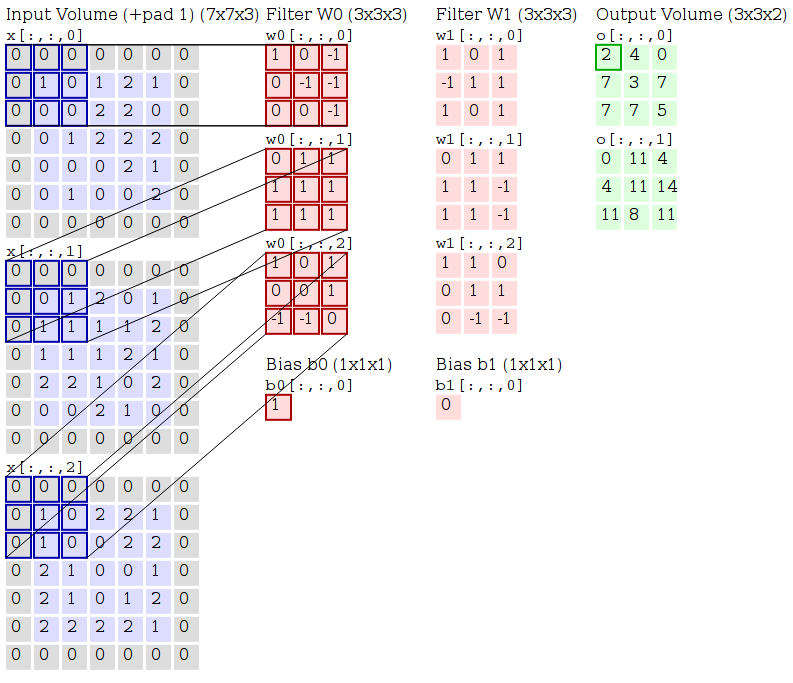
\includegraphics[scale=0.5]{Images/4_convolution.png}
%	\caption{Convolution algorithm with 2 filters of size 3x3, stride 2, zero padding 1}
%	\small Image adapted from \url{`http://cs231n.github.io/convolutional-networks/'}
%	\label{convnets-conv-alg}
%\end{figure}

%As shown in Figure \ref{convnets-conv-alg}, the convolution process starts from the top-left corner of the input volume. A subset of the image is taken at that location, with the same dimensions as the filter. The image subset and the filter are entry-wise multiplied and added together. A bias variable is added and an activation function applied as with fully connected layers. This result becomes the output of a single neuron of the convolutional layer. The filter is moved to the next location (depending on the size of the stride) to build the value of the next neuron.

Each filter of a convolutional layer outputs an array of reduced dimension compared to the input. These arrays are bound together to form a three-dimensional array, with depth dependent on the number of filters in the layer.

\subsection*{Zero padding}\label{convnets-pad}

During convolution, the filters are only placed within the boundaries of the input image, resulting in loss of dimension. For an input image with dimension $J \times K$ and a filter with dimension $M \times N$, the filter output will be of dimension $(J - M + 1)\times (K - N + 1)$.

\textit{Zero padding} surrounds the edges of the input image with $P$ layers of zeros, increasing the input dimension to  $(J+2P) \times (K+2P)$. When convolution takes place, the resulting image size will have dimension $(J+2P - M + 1) \times (K + 2P - N + 1)$. The value of $P$ can be set such that the convolution maintains the original image dimension.

\subsection*{Stride}\label{convnets-stride}

The dimension of the input images can be large, hence convolving filters at all possible locations results in lengthy training time. To reduce the number of resulting variables and improve training time, the filter can convolve at every $S$ location of the input. The magnitude of the filter movement is known as the \textit{stride}.

For an input image with dimension $J \times K$, a filter with dimension $M \times N$, with padding $P$ and stride $S$, the output given by convolution will have dimension $\left(\left\lfloor (J + 2P - M)/S\right\rfloor + 1\right) \times \left(\left\lfloor (K + 2P - N)/S \right\rfloor + 1\right)$.

\section{Pooling layers}\label{convnets-pool}

Convolutional layers are followed by pooling layers to reduce dimensionality of the data \cite{ADeshpande2016}. A sliding window of size $M\times M$ and stride $S$ is applied to the top-left of the image input and moves across the image similarly to the convolutional layers. At each location, the pooling layer outputs a single value which collectively form a matrix of reduced dimension to the input. For \textit{max pooling}, the values output are the maximum values of all inputs in each sliding window.

Max pooling is a preferred pooling method as it emphasises features of interest located by the previous convolutional layer. The algorithm is only interested in gathering information for classification and does not need the location to be highly specific. To improve computation time, it is advantageous to remove a large number of variables, while retaining variables that identify significant features.

\section{ReLU activation}\label{convnets-act}

The ReLU activation function, as defined in Section \ref{nnets-act}, is frequently used for  convolutional neural networks. Computation time can become very large as there are a large number of variables. The ReLU function can be computed very quickly and so is a common choice for convolutional neural networks \cite{ADeshpande2016}. Additionally, the ReLU activation function is also able to avoid the vanishing gradient problem (see Section \ref{nnet-vanishinggradprob}).


%Convolutional Neural Networks are very similar to traditional neural networks, but make the assumption that the input data are images.
%The neurons of a convNet are arranged in 3D. 
%http://cs231n.github.io/convolutional-networks/
%
%Input layer: raw pixel values, with width, height and color channels
%Conv layer: Compute output for regions of input. Each computes a dot product between weights and a region that they are connected to.
%ReLU: elementwise activation function.
%Pool: downsampling
%FC - fully connected: each neuron here is connected to all previous.
%
%Conv layer has a set of learnable filters. The filter might have only a small size, but will slide (convolve) across the image, computing dot products at each position.

%https://stats.stackexchange.com/questions/154879/a-list-of-cost-functions-used-in-neural-networks-alongside-applications
%https://pappubahry.com/misc/neural/nielsen_1/
% http://neuralnetworksanddeeplearning.com/

%Good animated representation: https://ujjwalkarn.me/2016/08/11/intuitive-explanation-convnets/
%
%https://medium.com/technologymadeeasy/the-best-explanation-of-convolutional-neural-networks-on-the-internet-fbb8b1ad5df8
%
%https://tensorflow.rstudio.com/tensorflow/articles/tutorial_mnist_beginners.html
%
%https://adeshpande3.github.io/A-Beginner%27s-Guide-To-Understanding-Convolutional-Neural-Networks-Part-2/
%
%https://tech.hbc.com/2016-05-18-fully-connected-to-convolutional-conversion.html


%\section{R-CNN}
%Purpose is to take in an image, and draw bounding boxes over all of the objects. Train to find 4D output (x, y, width, height) of object. Use L2 distance loss between prediction and 'ground truth'.
%
%Done by attaching a fully connected layer to the last conv layer. Separate classification layers and box coord layers. 
%Accuracy determined by Intersection over Union (ioU) area. 






%%%%%%%%%%%%%%%%%%%%%%%%%%%%%%%%%%%%%%%%%%%%%%%%%%%%%%%%%%%%%%%%%%%%%%%%%%%

%\clearpage

\addcontentsline{toc}{chapter}{References}

\bibliographystyle{apalike}
\bibliography{bibliography.bib}

%\bibliographystyle{apacite}
%\bibliography{mybib.bib}

